\documentclass[10pt,onecolumn]{witseiepaper}

\usepackage{KJN}
\usepackage{multicol}
\usepackage{chngcntr}

\ifpdf
\pdfinfo{
/Title (ELEN4012 - Feature Based Automatic Modulation Classification)
/Author (Jacques Visser and Anthony Farquharson)
}
\fi

\begin{document}

\title{ELEN4012 - Feature Based Automatic Modulation Classification}

\author{Jacques Visser and Anthony Farquharson
\thanks{School of Electrical \& Information Engineering, University of the
Witwatersrand, Private Bag 3, 2050, Johannesburg, South Africa}
}

% TODO Rewrite abstract once the rest of the contents are figured out.
\abstract{Automatic modulation classification involves identifying the modulation scheme used in a signal without the decision being guided by an operator. This report covers a preliminary investigation into the design and implementation of such a system. An overview of the relevant literature is presented and proposals are made regarding the details of the implementation and testing of such a system using and Ettus USRP.}

\keywords{modulation, classification, USRP, UHD}

\maketitle
\thispagestyle{empty}\pagestyle{empty}
\begin{multicols}{2}

\section{INTRODUCTION}
% TODO How does one even write an introduction?
% mention USRP's and define the term
% Also UHD

\section{LITERATURE SURVEY}
Zhu and Nandi identify three major approaches to automatic modulation classification in \textit{Automatic Modulation Classification: Principles, Algorithms and Applications} \cite{zhu2014automatic}; likelihood-based, distribution-test-based and feature-based. These are briefly detailed below.

	\subsection{Likelihood Based Classification}
	Likelihood based automatic modulation classification hinges on a Bayesian approach wherein various hypotheses regarding the likelihood of a signal conforming to a single modulation scheme are successively refined \cite{zhu2014automatic}. This approach is very popular as it results in optimal classification of modulation schemes \cite{zhu2014automatic}.

	This approach depends highly on knowledge of the channel and is characterized by a high computational complexity \cite{zhu2014automatic}. 

	\subsection{Distribution Test Based Classification}
	As the name suggests, distribution test-based modulation classifiers compare the statistical distribution of samples from a received distribution to known distributions to identify the modulation scheme \cite{zhu2014automatic}. Comparison to known distributions is generally done using a Kolmogorov-Smirnoff test which evaluates the goodness-of-fit between two distributions \cite{urriza2011computationally}.


	\subsection{Feature Based Classification}
	\label{sec:features}
	Feature based AMC has been shown to be non-ideal, but significantly less computationally intensive \cite{zhu2014automatic} than the aforementioned methods.

	There are again three major approaches to feature-based AMC. These make use of features derived from either the signal spectrum, the wavelet transform of the signal or high-order statistical representations of the signal \cite{zhu2014automatic}. 
	
	The classification of analog modulation schemes using spectral features is well documented by Zhu and Nandi \cite{zhu2014automatic} as well as Azzouz and Nandi \cite{azzouz2013automatic}. They make use of nine features, which are as follows:

	\begin{enumerate}
		\item $\gamma_{max}$: Maximum value of Power Spectral Density 
		\item $\sigma_{ap}$: Standard deviation of the absolute value of the non-linear component of the instantaneous phase.
		\item $\sigma_{dp}$: Standard deviation of the non-linear component of the direct instantaneous phase.
		\item $P$: Spectrum symmetry
		\item $\sigma_{aa}$: Standard deviation of the absolute value of the normalized and centered instantaneous amplitude
		\item $\sigma_{af}$: Standard deviation of the absolute value of the normalized and centered instantaneous frequency
		\item $\sigma_{a}$: Standard deviation of the normalized and centered instantaneous amplitude
		\item $\mu_{42}^{a}$: Kurtosis of the normalized and centered instantaneous amplitude
		\item $\mu_{42}^{f}$: Kurtosis of the normalized and centered instantaneous frequency
	\end{enumerate}

	The formulae for the computation of these features can be found in either \textit{Automatic Modulation Classification: Principles, Algorithms and Applications} by Zhu and Nandi \cite{zhu2014automatic} or \textit{Automatic modulation recognition of communication signals} by Azzouz and Nandi \cite{azzouz2013automatic}, and are omitted here for brevity.
	
\section{EXISTING APPLICATIONS OF AMC}
% TODO: Existing Applications
		% jamming, listening in on communications
		% cognative radio, effective use of bandwith
		% aircraft monitoring
Automatic modulation classification finds it's use in a variety of both civilian and military applications. 

In the sphere of signal jamming it is often useful to know the modulation scheme which is to be jammed. The jamming signal can be adapted to avoid non-offending broadcasts and use a minimum amount of power without compromising efficacy \cite{azzouz2013automatic}.

Cognitive radio, although nebulous, involves




\section{SOLUTION SELECTION}
	The selection of one of the three major types of modulation classification is motivated by the ease by which it can be practically implemented with the tools available and the time available for it's implementation. 
	This being the case, the spectral feature-based approach was chosen. It has a relatively low computational complexity and previous work has been done on the subject. This approach fulfills the requirements of being able to detect some digital- all major analog modulation schemes.

	However, if there is enough time available, the system could be extended, making use of some distribution test-based classification techniques in order to classify a larger range of digital modulation schemes.

\section{DEVELOPMENT METHODOLOGY} 
	For this project it has been deemed appropriate to make use of the incremental build-model of software development. This stresses small iterations of the analysis, design, code and test cycle- basically small waterfall development cycles \cite{incremental_model, waterfall_model}. The smaller segments make testing, debugging and risk management easier.

	Tracking of tasks will be done with Trello \cite{trello}, in Kanban style, with each card representing a single cycle\cite{kanban_model}. Cards move between three lists: 'Pending', 'In Progress' and 'Completed'.

\section{IMPLEMENTATION OVERVIEW}

	\subsection{Software}
		The software to be developed forms the core part of this system. It makes use of various libraries and frameworks to form a cohesive and efficient whole. 

		\subsubsection{Basic Software Structure}
			Due to the computationally intensive and time-dependent nature of the system, the software would have to be threaded, with each major component running on it's own thread.

			The software would consist of various components centered around a main control loop. The USRP Hardware Driver (UHD), run in it's own thread, passes the signal to the central control structure, which filters the signal and passes it to various feature extraction functions, all run in parallel. These functions deliver the features that have been extracted form the signal to a classifier which finally determines the modulation scheme used. This process is represented as a flow diagram in Figure \ref{fig:sw_overview}. The Feature extraction process is shown in Appendix \ref{app:feature} and discussed in Section \ref{sec:feat_fun}.

			\begin{figure}[h!]
				\centering
				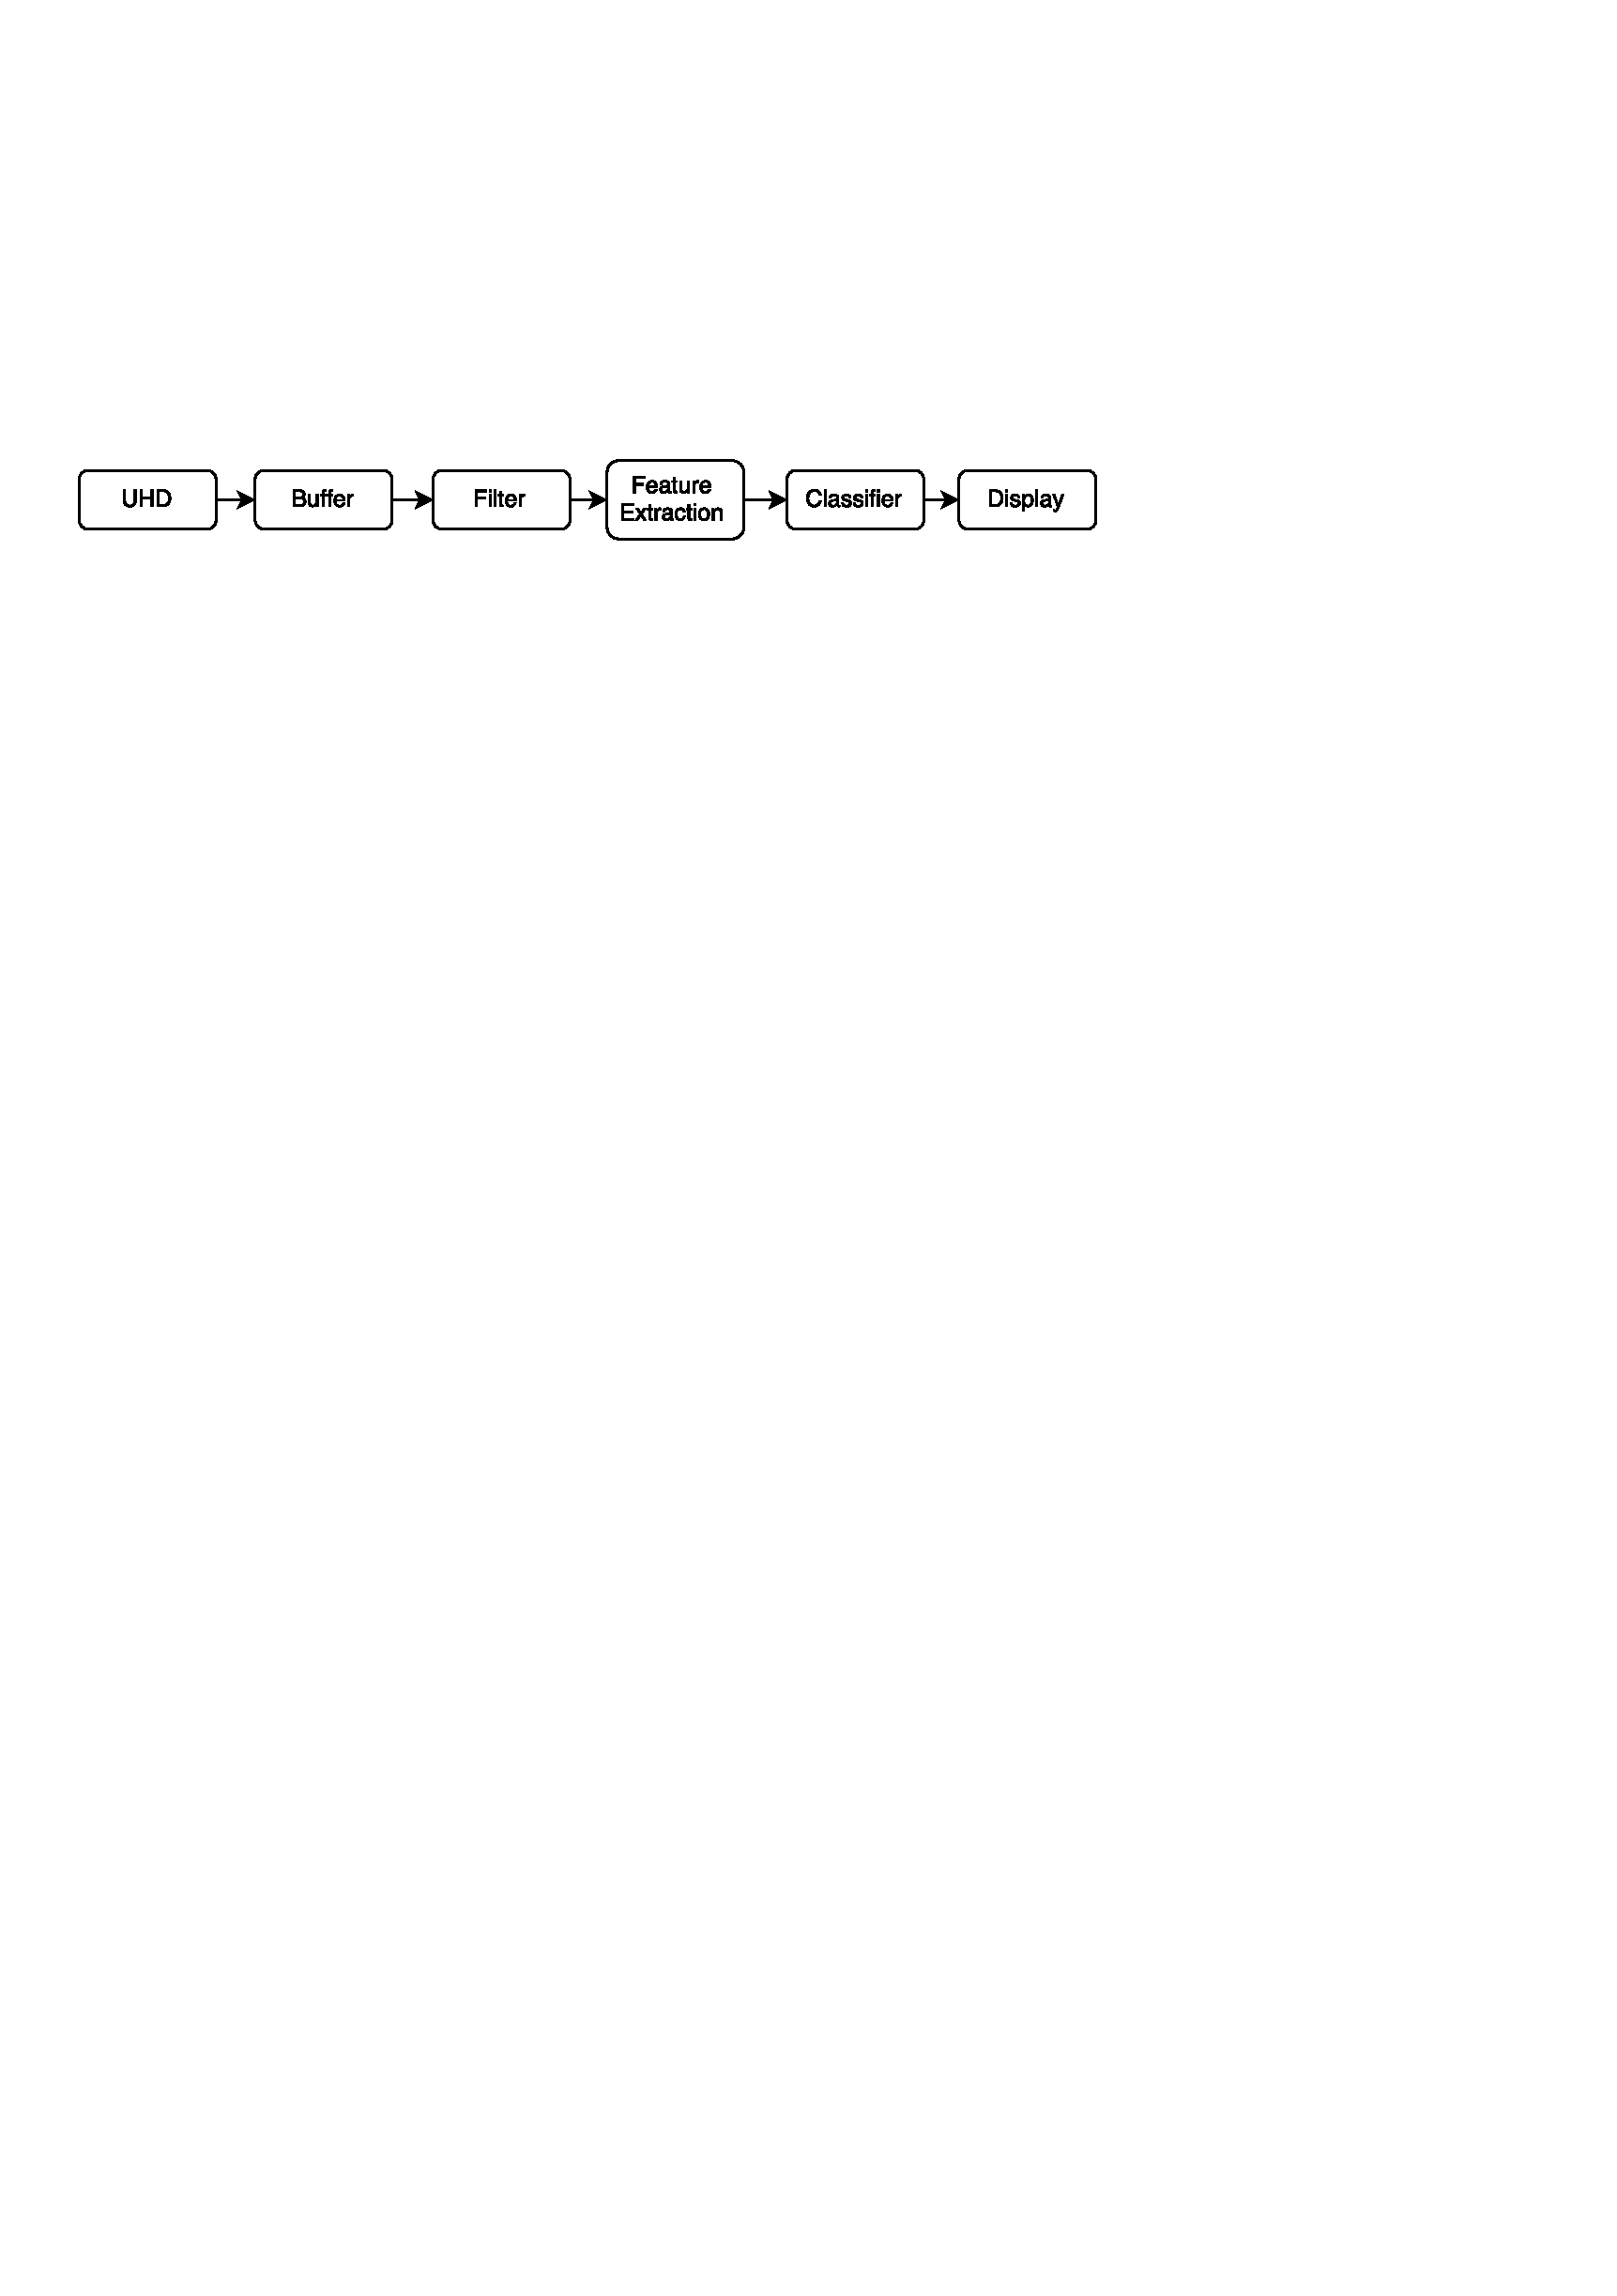
\includegraphics[trim=1.2cm 31.5cm 9cm 8cm, clip=true,width=0.5\textwidth]{small.pdf}
				\caption{Overview of the modulation classification process}
				\label{fig:sw_overview}
			\end{figure}

		\subsubsection{Libraries and API's}
			Due to the complicated nature of the software implementation, all of the components will not be locally developed. Rather, various API's and libraries will be used.

			Firstly, the Ettus USRP Hardware Driver's (UHD) C++ API will be used for communication with the USRP. This is a free \& open source piece of software released under the GPLv3 license \cite{uhd_license}, and is thus free to be used for a project such as this.

			In order to spectrally analyze the incoming signal the FFTW3 library is to be used. FFTW3 is an open-source C library developed by Matteo Frigo and Steven G. Johnson. It is available under the GPLv3 license \cite{fftw3_license}.

			For displaying graphical information SFML (Simple and Fast Multimedia Library) will be used. This is distributed under the zlib/libpng License and may thus be freely used in a project such as this \cite{sfml_license}.

			Creation of a gui and the display of information is to be done using the QT framework and QCustomPlot. These are distributed under the GTKv3 license \cite{qt_license, qcustomplot_license}. Furthermore, testing and QA will be done with QT Test simply due to convenience.

			For threading and other miscellaneous functions the C++ 11 Standard library will be used. GNU libstdc++ which is used with GCC is distributed under the GPLv3 license.

		\subsubsection{Build System}
			Due to the open-source nature and wide availability of the libraries and API's used in this project the software produced will be able to run on various platforms. To fully support this the CMake build-system-generator will be used so that this project may easily be compiled on various platforms.

			CMake is distributed under the BSD 3-Clause license \cite{cmake_license} and it can thus be distributed with and used in this project.

	\subsection{Feature Extraction}
		\label{sec:feat_fun}
		Individual functions will have to be developed for the extraction of each of the nine features mentioned in section \ref{sec:features}. Some of these features incorporate common data, thus the process of feature extraction may be accelerated by doing the computation thereof only once.

		A spectral representation of the signal is used in the process of obtaining most of the features. This is computed with an FFT using the FFTW3 library. 
		
		To obtain the instantaneous phase of the signal, the negative portion of the spectral representation of the signal is to be removed and an IFFT is to be performed \cite{picinbono1997instantaneous}. Following this, phase unwrapping must be performed \cite{park2009introduction, picinbono1997instantaneous}.

		The Instantaneous frequency of the signal may then be obtained from the instantaneous phase by differentiation \cite{park2009introduction}.

		This results in a complex series of events. They are shown in sequence as a flow diagram in Appendix \ref{app:feature}, Figure \ref{fig:feature}.

	\subsection{Signal Filtering}
		Filtering of the input signal to isolate the bandwidth in which a single signal exists will be done entirely digitally, independant of the USRP.

		Filtering in this context is a delicate process; phase distortion will negatively affect the results as many of the features are dependant on the non-linear portion of the phase only. 
		Thus it is important to implement zero-phase digital filtering.
		This may be done by either performing forward and reverse filtering or by selecting an FIR filter with a vary flat phase response \cite{sundararajan2003digital}.

		The former option would require buffering a large portion of the signal, but might yield better results than the latter. This trade-off, as well as selecting the bandwidth of the band-pass filter to be used is still under investigation.

		Filtering will be implemented by convolution as the alternative, multiplication in the Fourier domain, would result in an extra step in feature extraction: finding the magnitude of the resulting signal after performing the IFFT. (See Appendix \ref{app:feature} for more information)

	\subsection{Classifier}
	K-nearest neighbors

	\subsection{Hardware}
		The practical implementation of this project will require at least two USRP devices. The first of which will be used for receiving radio signals, the modulation of which is to be classified. The second will be used to generate modulated signals in order to practically test the operation of the system. Seeing as Wits has these available, no charges would be incurred.

		To avoid significant effort in compiling and installation of the USRP Hardware Driver (UHD) two computers running Linux natively will be required. The team-members' laptops will be used for this purpose.

\section{PROPOSED TESTING PROCEDURE}
	Basic unit testing and incremental integration testing of the application is to be done with the QT framework's QTest. Functional testing will is to be implemented to train the classifier. System testing is to be done with practical signals to evaluate the effectiveness of the system.
	\subsection{Functional Testing}
		The functional testing will involve supplying signals to the system through a mocking framework, rather than the UHD driver. In so doing, the classifier can be trained on ideal signals. Noise may be introduced to signals of various lengths to evaluate the system's functioning under a variety of conditions.

	\subsection{Practical Testing}
		Practical testing is to be done with signals generated using another USRP and GNURadio. This will allow for comparing the ideal functioning of the system, and thus spectral feature-based modulation classification in general, to it's real world operation.

\end{multicols}
	\begin{figure}[h]
		\centering
		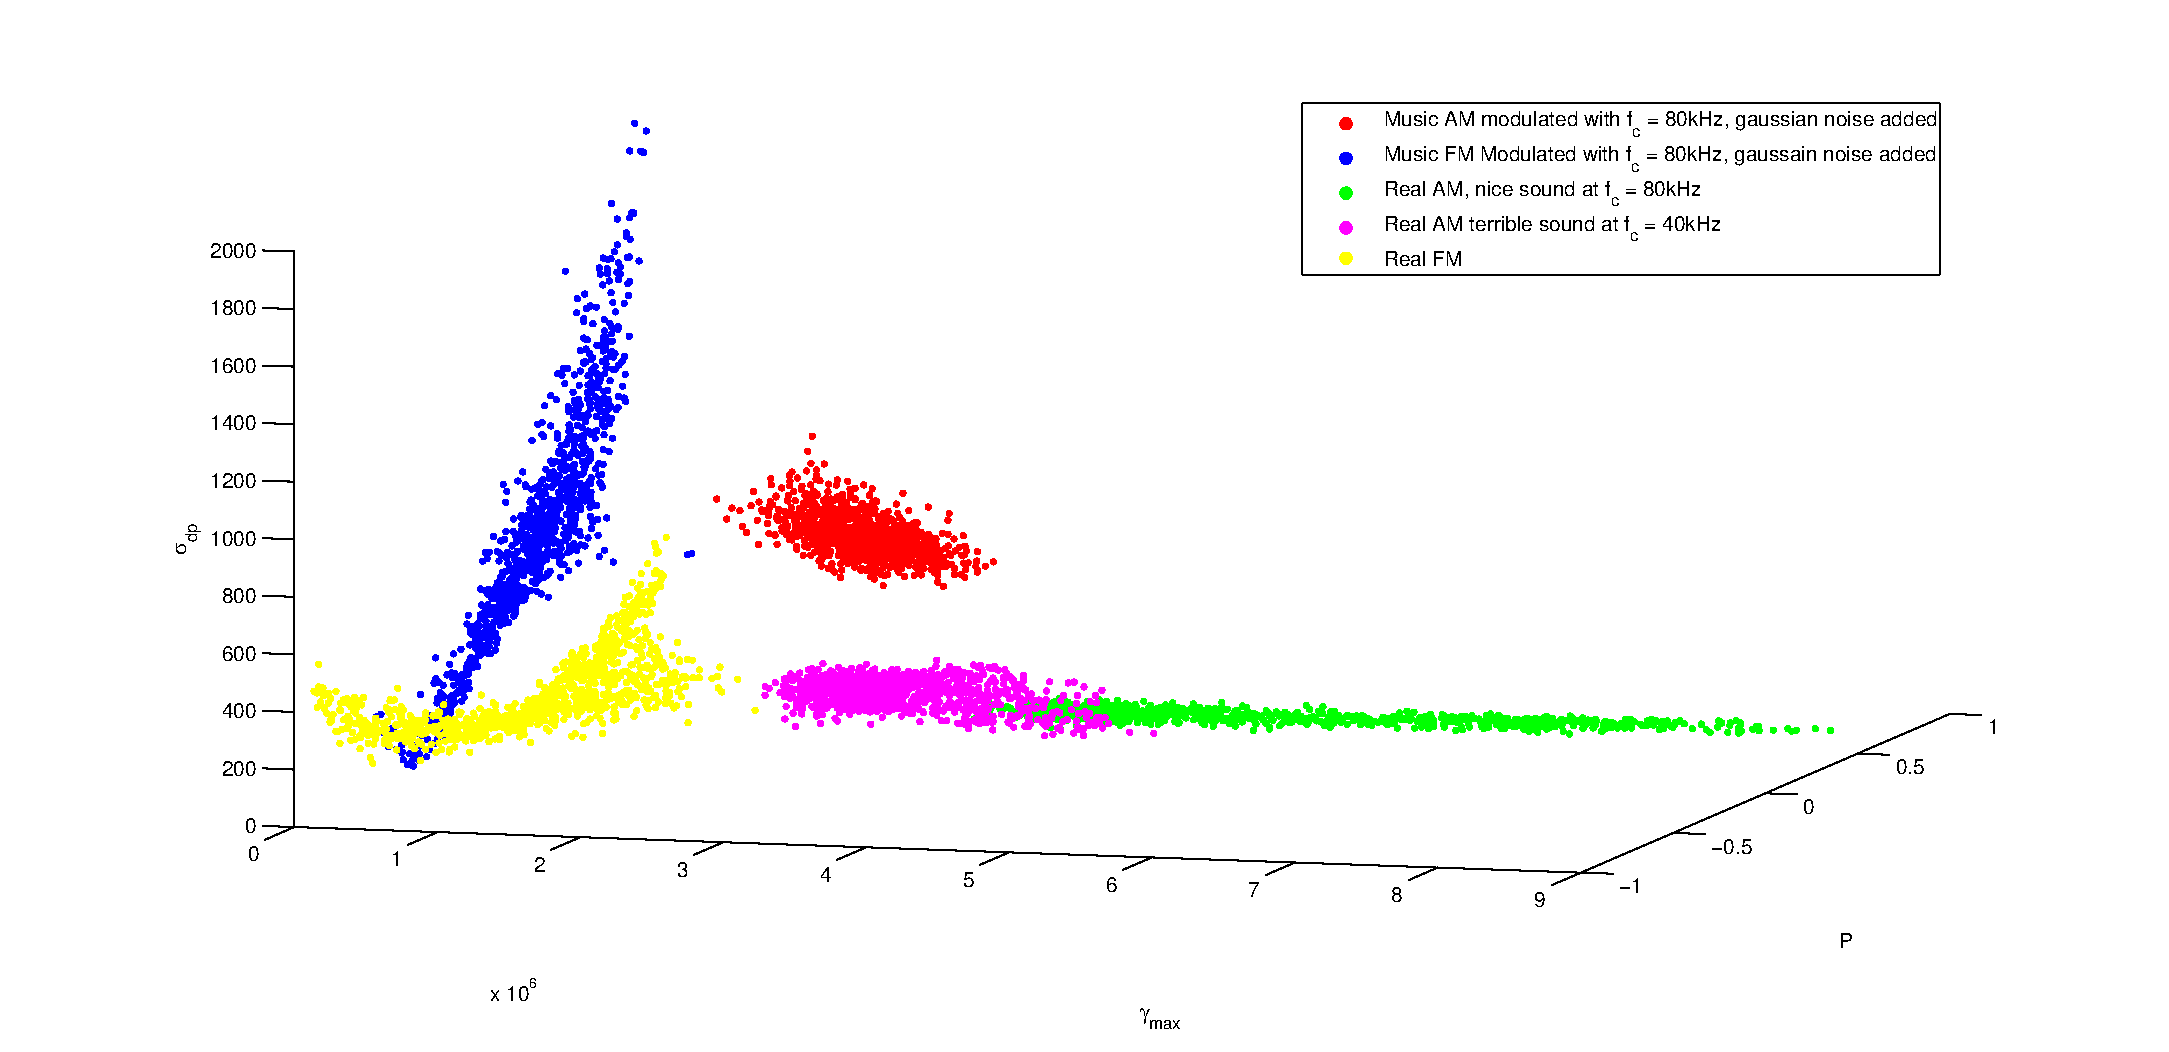
\includegraphics[width=1\textwidth]{plot0.eps}
		\caption{Plot of $\sigma_{dp}$ vs. $\gamma_{max}$ vs. $P$ for various AM and FM signals}
		\label{fig:plot0}
	\end{figure}
\begin{multicols}{2}

\section{PRELIMINARY RESULTS}
	Simple testing of the feature-based AMC algorithm was performed in MATLAB with a limited number of features. The results are promising, showing a clear separation between different modulation schemes. This can be seen in Figure \ref{fig:plot0}. 

	The marked clustering of the results show that it is indeed possible to make use of a simple threshold-based decision-tree classifier. Making use of such a classifier, however, would require intense interaction with the application to set the appropriate thresholds. Thus it has been deemed appropriate to make use of a K-Nearest-Neighbor clustering algorithm so as to maximise the application's autonomy and extensibility.

\section{CONCLUSION}

% TODO conclusion

\bibliographystyle{witseie}
\bibliography{prelim} 
\end{multicols}
\newpage

\appendix
\counterwithin{figure}{section}
\section{Feature Extraction Process}
\label{app:feature}
The process of feature extraction is fairly complex. It is presented as a flow graph in Figure \ref{fig:feature} below. Because of the nature of the process it is amenable to parallelization. This will be performed using the C++ 11 Standard threading library.

\begin{figure}[h!]
	\centering
	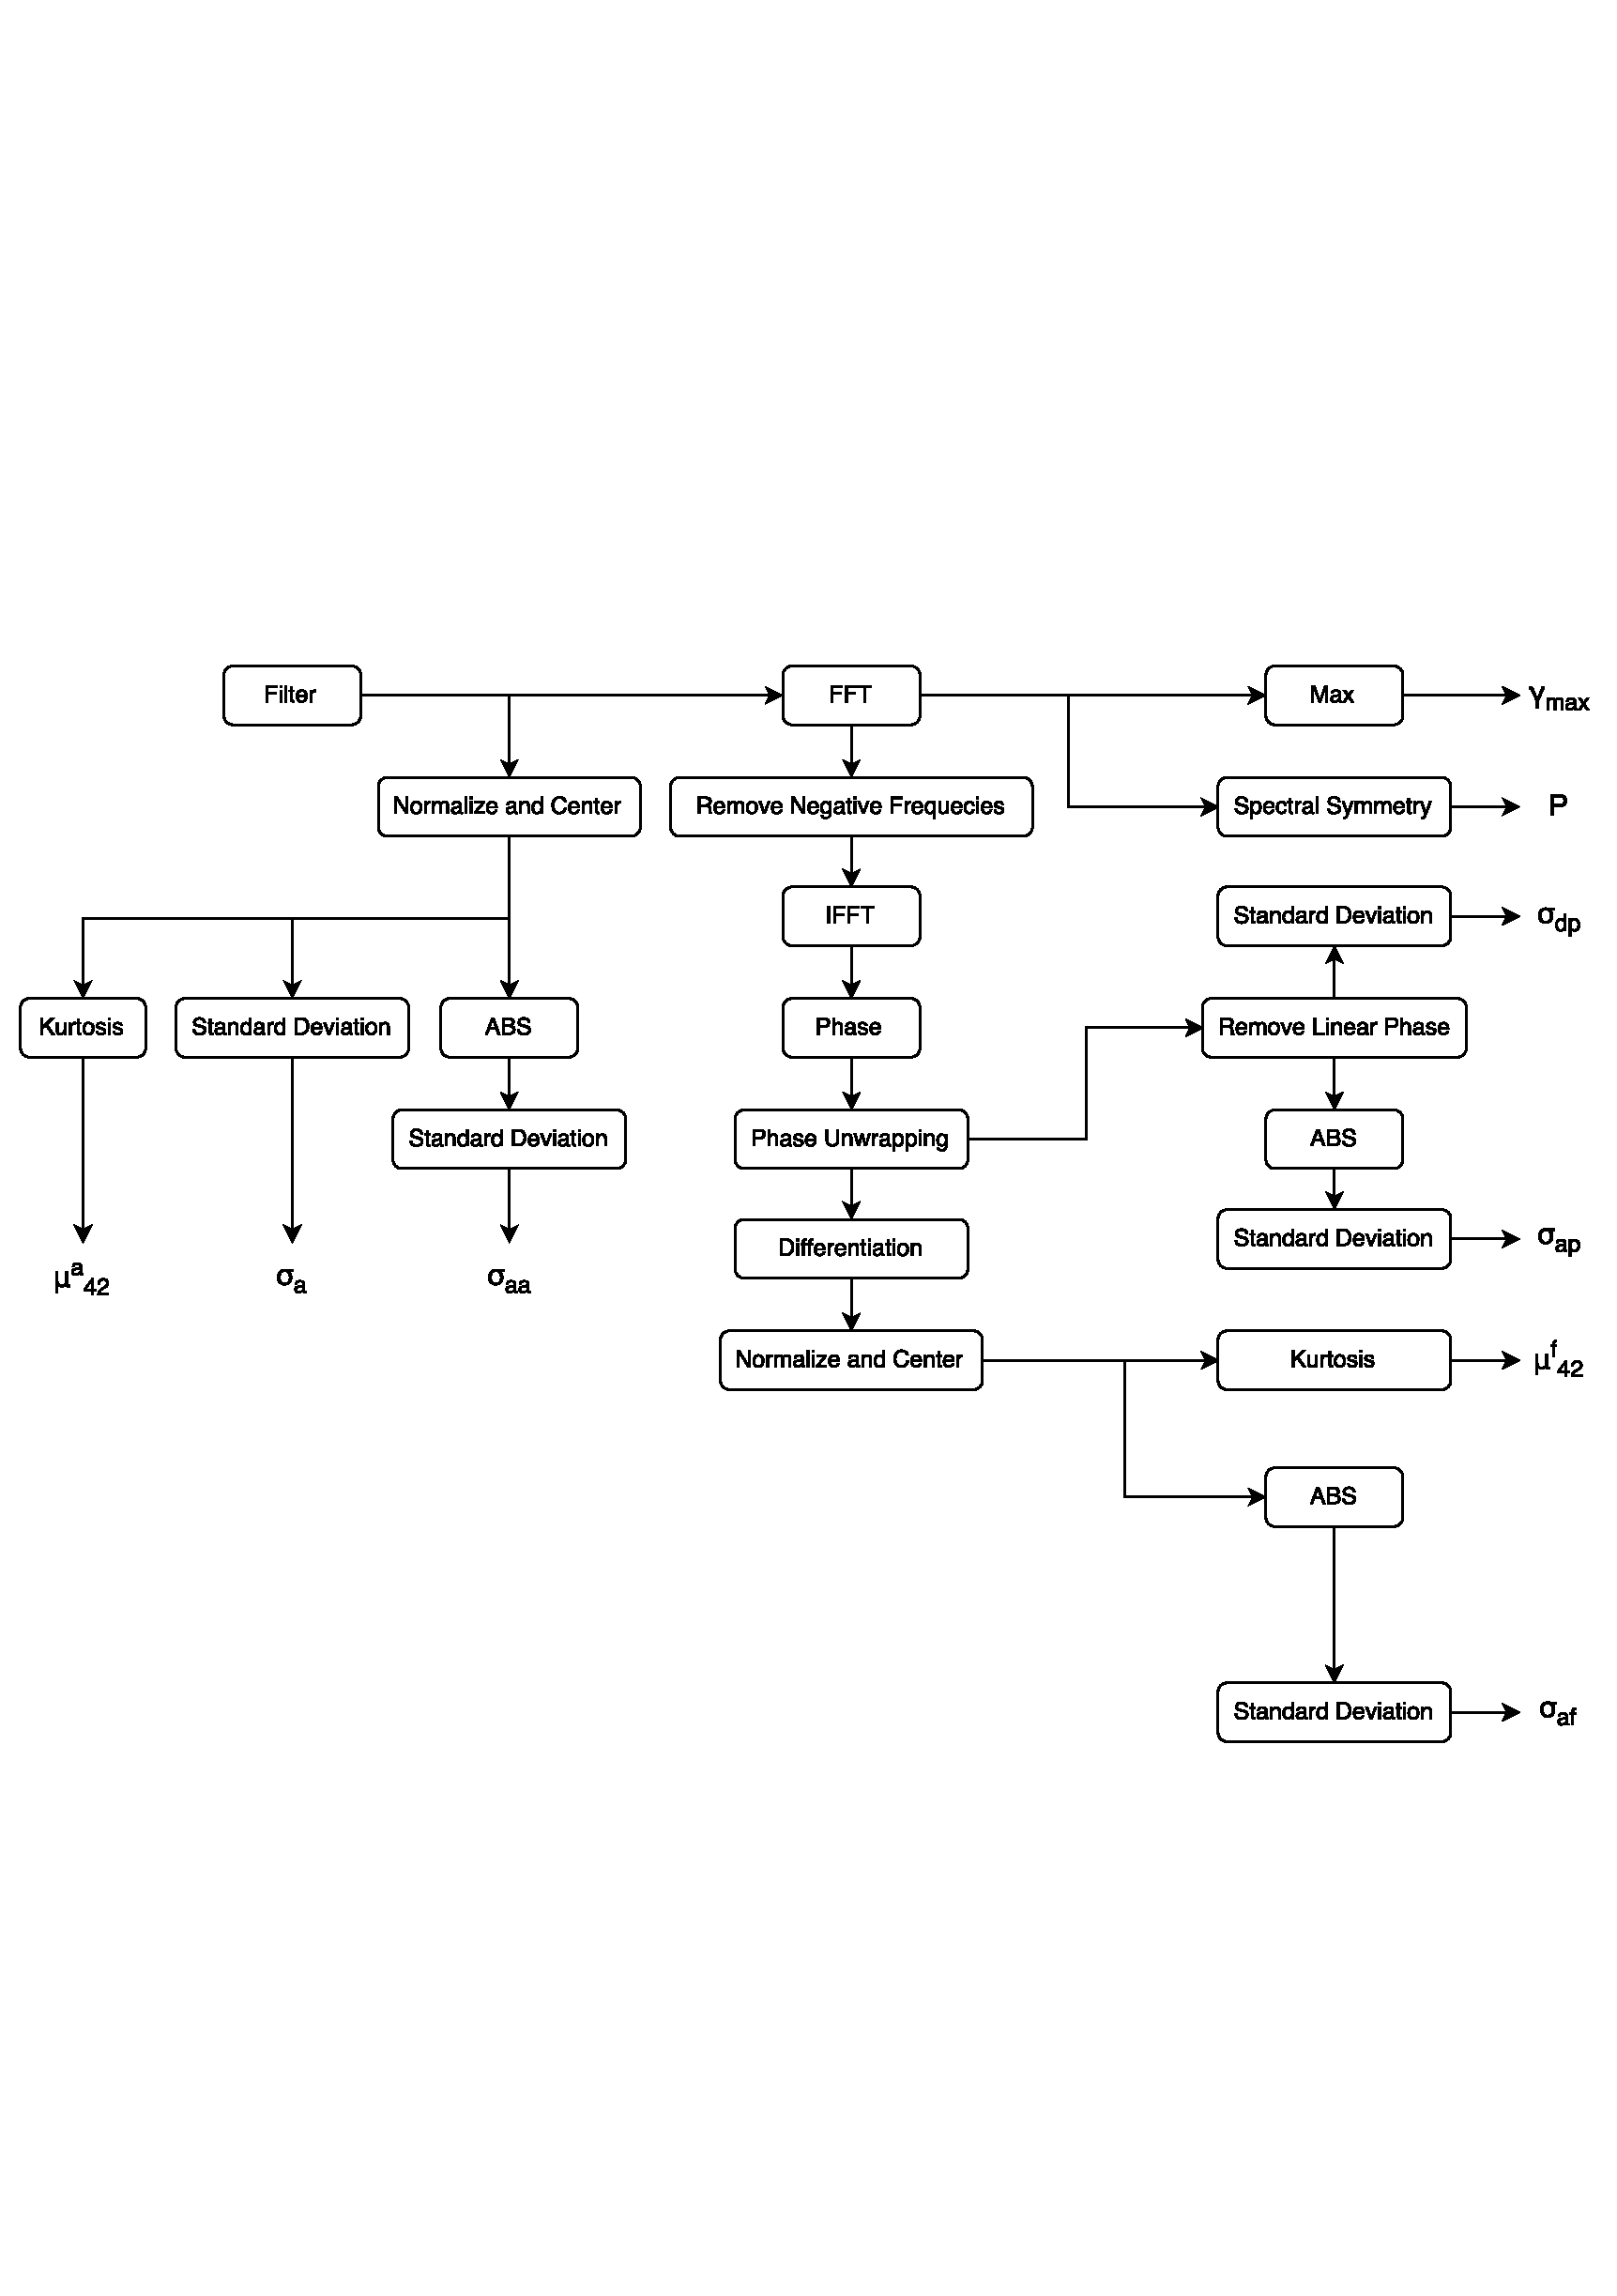
\includegraphics[trim=0cm 10cm 0cm 11cm, clip=true,width=0.8\textwidth]{large.pdf}
	\caption{Feature extraction process as a flow graph}
	\label{fig:feature}
\end{figure}

Filtering of the signal prior to feature extraction is done by means of convolution. The alternative, filtering by multiplication in the Fourier domain, would imply that both the phase and magnitude of the output of the IFFT in Figure \ref{fig:feature} need to be found. The magnitude found here is equivalent to the input of the FFT. This approach would not only impact the accuracy of the instantaneous amplitude measure, but also introduce another unnecessary operation.

% "It don't matter, Jacques, I live my life lo-fi and noisy." - Anthony

\end{document}

